\chapter{Memory Management as a Service}
\label{chap:service}
The service layer, positioned above the OS layer, plays a pivotal role in facilitating efficient and seamless memory sharing across multiple computing and memory nodes within a disaggregated architecture. As application software, it provides greater flexibility than the operating system, allowing for a variety of services to be offered to applications. These adaptable services enable applications to choose options best suited to their specific needs. However, this requires that the storage and compute are easily decoupled, otherwise the application developers will need to spend enormous effort to modify the application for it to use memory management service. 

Serverless architecture offer on-demand elasticity of compute and storage and decouples them logically. Recent work on serverless analytics has demonstrated the benefit of using serverless architecture for resource- and cost-efficient data analytics. The key idea of serverless analytics is to use a remote low-latency, high-throughput shared far-memory system for (1) inter-task communication and (2) for multi-stage jobs, storing intermediate data beyond the lifetime of the task that produced the data. This makes it a perfect target for disaggregate memory since compute and memory are decoupled logically when the serverless task is assigned.

Designing a memory management service is a non-trivial tasks. Our discussion begins with an outline of the essential requirements for such memory management services, focusing on the unique challenges introduced by disaggregation. We then highlight our current efforts to tackle these challenges and explore potential directions for future research in this rapidly evolving domain.

\paragraphb{Elasticity}  Memory usage in modern computing environments can be highly variable, with applications experiencing fluctuating memory demands~\cite{jiffy}. Elasticity allows the memory service to dynamically allocate and deallocate memory resources based on current requirements, optimizing resource utilization. In typical applications with dynamic memory requirements, such as data analytics, applications are organized into jobs that contain multiple tasks. Each task can be assigned to run on an arbitrary compute node. Each task communicates with the other using memory as intermediate storage. Previous solutions ~\cite{pocket} tend to allocate resources in a job granularity. Jobs specify their memory demands before the job is submitted and the system reserves the amount of memory for the entire job lifetime. The tradeoff between performance and resource utilization for such job-level resource allocation is indeed well studied in prior work ~\cite{jiffy}. On the one hand, if jobs specify an average demand of memory, the job will degrade as running out of memory will lead to swapping data out to slower storage medium (e.g. S3 storage), while on the other hand allocating at peak granularity will result in resource wastage.

\paragraphb{Isolation} The second requirement is the isolation between different compute tasks. Since multiple computing threads can be using the same disaggregated memory pool, it's essential to multiplex between applications to improve resource efficiency but at the same time keep the memory of different threads isolated from each other, which means that the memory usage of a particular application should not affect other existing applications. The number of tasks reading and writing to the shared disaggregated memory can change rapidly in serverless analytics which makes the problem even more severe.

\paragraphb{Lifetime management}
Decoupling compute tasks from their intermediate storage means that the tasks can fail independent of the intermediate data, therefore we need mechanisms for explicity lifetime management of intermediate data.

\paragraphb{Data repartitioning}
Decoupling tasks from their intermediate data also means that data partitioning upon elastic scaling of memory capacity becomes challenging, especially for certain data types used in serverless analytics (e.g. key-value store). If it's the application's responsibility to perform such repartitioning, it will involve large network transfers betweem compute tasks and the far memory system and massive read/write operations every time the capacity is scaled. What's more, the application need to implement different partitioning strategies for different kind of data structures used. Therefore, new mechansims to efficiently enable data partitioning within the far memory system is essential.


We present Jiffy, an elastic disaggregated-memory system for stateful serverless analytics. Jiffy allocates memory resources at the granularity of small fixed-size memory blocks - multiple memory blocks store intermediate data for individual tasks within a job. Jiffy design is motivated by virtual memory design in operating systems that also does memory allocation to individual process at the granularity of fixed-size memory blocks(pages). Jiffy adapts this design to stateful serverless analytics. Performing resource allocation at the granularity of small memory blocks allows Jiffy to elastically scale memory resources allocated to individual jobs without a priori knowledge of intermediate data sizes and to meet the instantaneous job demands at seconds timescales. As a result, Jiffy can efficiently multiplex the available faster memory capacity across concurrently running jobs, thus minimizing the overheads of reads and writes to significantly slower secondary storage (e.g., S3 or disaggregated storage)

\section{Elastic memory management for data analytics}
\begin{comment}
\begin{figure}[t]
    \centering
    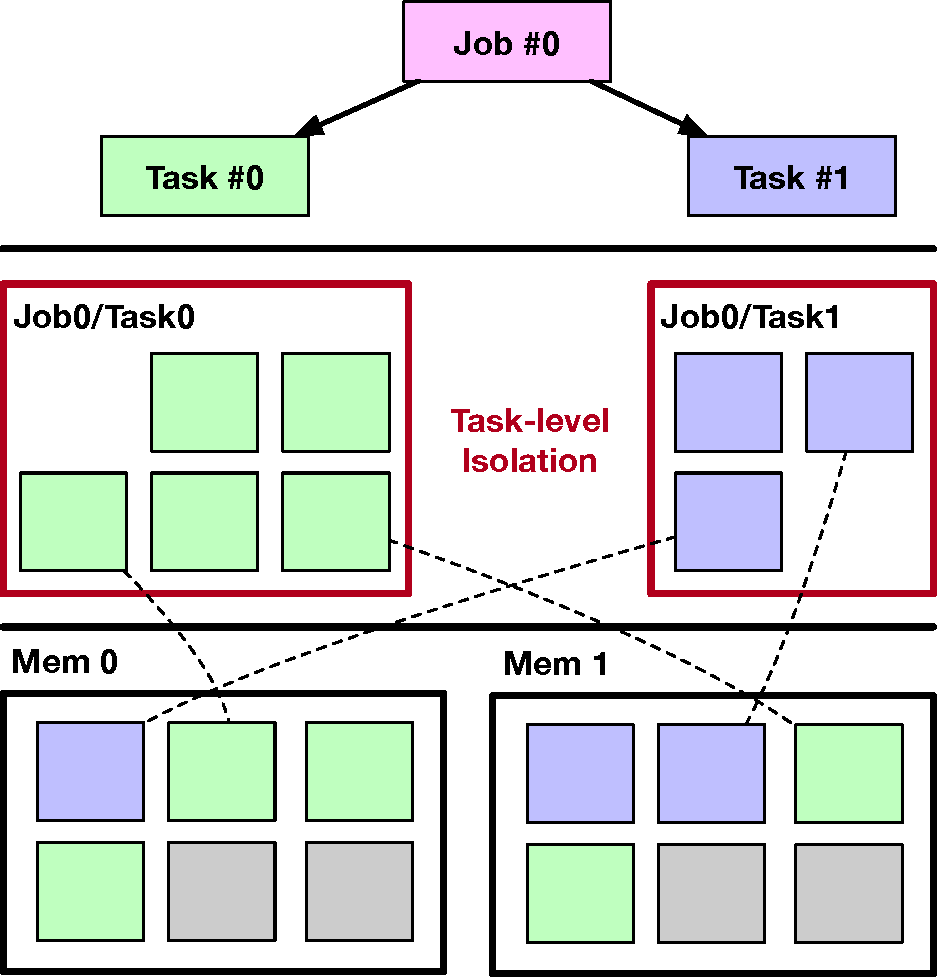
\includegraphics[width=0.6\columnwidth]{Jiffy.pdf}
    \caption{\textbf{Jiffy Overview.} Jiffy allocates memory resources individually for each task within a job. Memory is allocated in small, fixed-sized blocks to ensure elastic scaling of memory according to demand.} 
    \label{fig:jiffy} \vspace{-2.0em}
  \end{figure}
\end{comment}
Data analytics applications, which utilize disaggregated memory for inter-task communication and intermediate data storage, are becoming increasingly common. As discussed in ~\cite{starling, shuffling, pocket, cirrus}, these applications handle user requests in the form of jobs, each defining its memory needs upon creation. The dilemma of balancing performance with resource efficiency for job-level memory allocation has been extensively studied ~\cite{elasticquery, qoop}. If a job is based on average demand, performance may decline during peak demand periods due to inadequate memory, causing data spillage to slower secondary storage, such as SSDs. Conversely, allocating memory for peak demands leads to underutilization of resources when the actual demand is below peak. Evaluations on Snowflake's workload, as shown in ~\cite{elasticquery}, indicate a significant fluctuation in the ratio of peak to average demands, sometimes varying by two orders of magnitude within minutes.

In response to the challenges of dynamically allocating memory resources in data analytics applications, we have developed Jiffy~\cite{jiffy}, an elastic memory service tailored for disaggregated architectures. As shown in Figure \ref{fig:jiffy}, Jiffy allocates memory in small, fixed-size blocks, enabling the dynamic adjustment of memory allocation for individual jobs without prior knowledge of intermediate data sizes. Jiffy employs a hierarchical address space that reflects the structure of the analytics job, facilitating efficient management of the relationship between memory blocks and tasks while ensuring task-level isolation.

\section{Introduction}


Serverless architectures offer flexible compute and storage options, charging users for precise resource usage. Initially used for web microservices, IoT, and ETL tasks, recent advancements show their efficacy in data analytics. Serverless analytics leverage remote, high-throughput memory systems for inter-task communication and storing intermediate data. However, existing far-memory systems face limitations, allocating resources at the job level, leading to performance issues and underutilization.

To address this, we introduce Jiffy, an elastic far-memory system for stateful serverless analytics. Unlike conventional systems, Jiffy allocates memory in small, fixed-size blocks, enabling dynamic scaling and efficient resource utilization. This approach resolves challenges unique to serverless analytics, including task mapping, task isolation, and data lifetime management.

Our implementation of Jiffy features an intuitive API for seamless data manipulation. We demonstrate its versatility by implementing popular distributed frameworks like MapReduce, Dryad, StreamScope, and Piccolo. Evaluation against state-of-the-art systems indicates Jiffy’s superior resource utilization and application performance, achieving up to 3x better efficiency and 1.6–2.5x performance improvements.


\section{Motivation}
The leading system for stateful serverless analytics is Pocket, a distributed system designed for high-throughput, low-latency storage of intermediate data. Pocket effectively tackles several key challenges in stateful serverless analytics, including:

\paragraphb{Centralized management} Pocket's architecture features separate control, metadata, and data planes. While data storage is distributed across multiple servers, management functions are centralized, simplifying resource allocation and storage organization. A single metadata server can handle significant request loads, supporting thousands of serverless tasks.

\paragraphb{Multi-tiered data storage} Pocket's data plane stores job data across multiple servers and serves them via a key-value API. It supports storage across different tiers like DRAM, Flash, or HDD, enabling flexibility based on performance and cost constraints.

\paragraphb{Dynamic resource management} Pocket can scale memory capacity by adding or removing memory servers based on demand. The controller allocates resources for jobs and informs the metadata plane for proper data placement.

\paragraphb{Analytics execution with Pocket} Jobs interact with Pocket by registering with the control plane, specifying memory resources needed. The controller allocates resources and informs the metadata plane. Serverless tasks can access data directly from memory servers. Once a job finishes, it deregisters to release resources.

In our analysis, we focus on challenges in Pocket's resource allocation. Pocket allocates memory at the job level, which poses challenges in accurately predicting intermediate data sizes and leads to performance degradation or resource underutilization. This issue persists due to the dynamic nature of intermediate data sizes across different stages of execution.


\section{Jiffy Design}

\subsection{Overview}
Jiffy facilitates precise sharing of far-memory capacity among concurrent serverless analytics tasks for intermediate data storage. Drawing inspiration from virtual memory, Jiffy divides memory capacity into fixed-sized blocks, akin to virtual memory pages, and performs allocations at this granular level. This approach yields two key benefits: firstly, Jiffy can swiftly adapt to instantaneous job demands, adjusting capacity at the block level within seconds. Secondly, Jiffy doesn't necessitate prior knowledge of intermediate data sizes from jobs; instead, it dynamically manages resources as tasks write or delete data.

It's worth noting that multiplexing available memory capacity differs from merely scaling the memory pool's overall capacity. While prior systems like Pocket focus on the latter, adding or removing memory servers based on job arrivals or completions, Jiffy prioritizes efficient sharing of available capacity among concurrent jobs. This approach minimizes underutilization of existing capacity, a common issue in job-level resource allocation systems. Even during high memory capacity utilization, Jiffy can augment capacity by adding memory servers akin to Pocket. Notably, by efficiently multiplexing capacity across concurrent jobs, Jiffy reduces the need for frequent additions or removals of memory servers.

In addressing the challenges posed by serverless analytics, Jiffy implements hierarchical addressing, data lifetime management, and flexible data repartitioning. These mechanisms are discussed in detail in subsequent sections, with illustrative examples provided in Fig. 3, depicting a typical analytics job's execution plan organized as a directed acyclic graph (DAG) with computation tasks represented as serverless functions exchanging intermediate data via Jiffy.
\subsection{Hierarchical Addressing}

Analytics jobs typically follow a multi-stage or directed acyclic graph structure. In serverless analytics, where compute elasticity is integral, each job may entail tens to thousands of individual tasks. Consequently, achieving fine-grained resource allocation necessitates an efficient mechanism for maintaining an updated mapping between tasks and allocated memory blocks. Additionally, the rapidly changing number of tasks accessing shared memory underscores the importance of isolation at the task level to prevent performance degradation across jobs. In this context, Jiffy's hierarchical addressing system plays a crucial role.

Instead of relying on a network structure, Jiffy employs a hierarchical addressing mechanism tailored to the execution structure of analytics jobs. It organizes intermediate data within a virtual address hierarchy, reflecting the dependencies between tasks in the job's DAG. For instance, internal nodes represent tasks, while leaf nodes denote memory blocks storing intermediate data. The addressing scheme enables precise resource allocation at the task level, independent of other tasks, akin to virtual memory's process-level isolation.

This hierarchical addressing facilitates efficient management of resource allocations, ensuring that overflow into persistent storage doesn't impact the performance of other tasks. Each memory block, once allocated, remains dedicated to its task until explicitly released, guaranteeing isolation at the task level regardless of concurrency. This approach aligns with virtual memory principles, where each process enjoys its own address space, ensuring isolation at the process level.

Jiffy's design considers two key aspects. Firstly, resource allocation is decoupled from policy enforcement, allowing seamless integration of fairness algorithms atop Jiffy's allocation mechanism. Secondly, address translation, handled centrally, enables addressing for arbitrary DAGs without imposing limitations on execution structure complexity. While Jiffy's hierarchical addressing introduces complexity at the controller, its scalability is validated in our evaluation, accommodating realistic deployment demands.

Regarding block sizing, Jiffy's approach, akin to traditional virtual memory's page sizing, balances metadata overhead and memory utilization. Larger block sizes reduce per-block metadata, but may lead to data fragmentation, while smaller sizes optimize memory utilization at the expense of increased metadata overhead. Jiffy mitigates fragmentation via data repartitioning and allows block size configuration during initialization for compatibility with analytics frameworks.

Isolation granularity in Jiffy is task-level by default, but can be adjusted finer or coarser by adapting the hierarchy. For most analytics frameworks, task-level isolation suffices, but custom hierarchies can be created using Jiffy's API to tailor isolation to specific needs.
\subsection{Data Lifetime Management}
Existing far-memory systems for serverless analytics typically manage data lifetimes at the granularity of entire jobs, reclaiming storage only when a job explicitly deregisters. However, in serverless analytics, the intermediate data of a task is dissociated from its execution, residing in the far-memory system. This decoupling extends to fault domains: traditional mechanisms, such as reference counting, can result in dangling intermediate data if a task fails. To address this inefficiency, effective task-level data lifetime management mechanisms are required.

Jiffy tackles this challenge by integrating lease management mechanisms with hierarchical addressing. Each address-prefix in a job's hierarchical addressing is associated with a lease, and data remains in memory only as long as the lease is renewed. Consequently, jobs periodically renew leases for the address-prefixes of running tasks. Jiffy tracks lease renewal times for each node in the address hierarchy, updating them accordingly. Upon lease expiry, Jiffy reclaims allocated memory after flushing data to persistent storage, ensuring data integrity even in the event of network delays.

A novel aspect of Jiffy's lease management is its utilization of DAG-based hierarchical addressing to determine dependencies between leases. When a task renews its lease, Jiffy extends the renewal to the prefixes of tasks it depends on (parent nodes) and the prefixes of tasks dependent on it (descendant nodes), minimizing the number of renewal messages sent. This approach ensures that not only is a task's own data retained in memory while it's active, but also the data of tasks it depends on and tasks dependent on it. This mechanism strikes a balance between age-based eviction and explicit resource management, granting jobs control over resource lifetimes while tying resource fate to job status.

In an example scenario, task T7 periodically renews leases for its prefix during execution, ensuring the retention of intermediate data for blocks under it in memory. Lease renewals for T7's prefix also extend to its parent and descendant tasks, ensuring continuity of data access. However, leases for inactive tasks are not automatically renewed, preventing unnecessary resource retention.

Lease duration in Jiffy involves a tradeoff between control plane bandwidth and system utilization. Longer lease durations reduce network traffic but may lead to underutilization of resources until leases expire. Jiffy's sensitivity to lease durations is evaluated in the subsequent section.




\subsection{Flexible Data Repartitioning}
Decoupling compute tasks from their intermediate data in serverless analytics poses a challenge in achieving memory elasticity efficiently at fine granularities. When memory is allocated or deallocated to a task, repartitioning the intermediate data across the remaining memory blocks becomes necessary. However, due to the decoupling and the high concurrency of tasks, it's impractical to expect the application to handle this repartitioning. For instance, in many existing serverless analytics systems, key-value stores are used to store intermediate data. If a compute task were to handle repartitioning upon memory scaling, it would need to fetch key-value pairs from the store over the network, compute new data partitions, and then write back the data, incurring significant network latency and bandwidth overheads.

As discussed in §5, Jiffy already incorporates standard data structures utilized in data analytics frameworks, ranging from files to key-value pairs to queues. Analytics jobs leveraging these data structures can delegate repartitioning of intermediate data upon resource allocation/deallocation to Jiffy. Each block allocated to a Jiffy data structure monitors the fraction of memory capacity currently utilized for data storage. When usage surpasses a high threshold, Jiffy allocates a new block to the corresponding address-prefix. Subsequently, the overloaded block initiates data structure-specific repartitioning to migrate some data to the new block. Conversely, when block usage falls below a low threshold, Jiffy identifies another block with low usage within the address-prefix for potential data merging. The block then undergoes the necessary repartitioning before deallocation by Jiffy.

By tasking the target block with repartitioning instead of the compute task, Jiffy circumvents network and computational overheads for the task itself. Furthermore, data repartitioning in Jiffy occurs asynchronously, enabling data access operations across data structure blocks to proceed even during repartitioning. This ensures minimal impact on application performance due to repartitioning.

The data structures integrated into Jiffy enable the implementation of serverless versions of various powerful distributed programming frameworks, including MapReduce, Dryad, StreamScope, and Piccolo. Notably, the simplicity of repartitioning mechanisms required by analytics framework data structures allows serverless applications utilizing these programming models to seamlessly run on Jiffy and leverage its adaptable data repartitioning without any modifications.

Regarding thresholds for elastic scaling, the high and low thresholds in Jiffy present a tradeoff between data plane network bandwidth and task performance on one side and system utilization on the other. Optimizing these thresholds balances the frequency of elastic scaling triggers and system utilization efficiency. We evaluate Jiffy's sensitivity to threshold selections in §6.6.

\section{Applications and Evaluation}
\section{Related Work}
\section{Conclusion}